\documentclass[a4paper, 12pt]{article}
\usepackage[frenchb]{babel}
\usepackage[utf8]{inputenc}
\usepackage[T1]{fontenc}
\usepackage{times}
\usepackage{lmodern}
\usepackage{graphicx}
\usepackage{parskip}
\usepackage{float}
\usepackage{multicol}
\usepackage[colorlinks = true, linkcolor = blue, urlcolor = blue, citecolor = blue, anchorcolor = blue]{hyperref}

\newcommand{\git}{\texttt{git}}
\renewcommand{\familydefault}{\sfdefault}

\floatplacement{figure}{H}

\addtolength{\parskip}{\baselineskip}
\setlength{\parindent}{15pt}
\graphicspath{{images/}}
\begin{document}
%!TEX root = rapport_ir1.tex
\newcommand{\HRule}{\rule{\linewidth}{0.5mm}}
\begin{titlepage}
\begin{center}


\hfill\textsc{\LARGE{Paul OLLIVIER}\\[0.4cm]
\hfill\href{mailto:contact@paulollivier.fr}{\texttt{contact@paulollivier.fr}}}

\vfill

% Title
\HRule \\[0.4cm]
{ \huge \bfseries Ullink: une entreprise en pleine expansion\\[0.4cm] }

\HRule \\[1.5cm]
\vfill

% Bottom of the page
{\large 08/2013 \hfill Informatique et Réseau 1\textsuperscript{ère} année}

\end{center}
\end{titlepage}

\pagebreak

\section*{Remerciements}
\addcontentsline{toc}{section}{Remerciements}
Je remercie l'ensemble de l'équipe tutorale de l'Esipe, particulièrement Philippe FINKEL, mon tuteur enseignant. Je remercie également mes collègues d'Ullink, avec mention spéciale pour mon tuteur ingénieur, Nicolas CHEVALIER, et enfin Laurent BARBISAN, qui m'a beaucoup aidé.

\pagebreak

\section*{Introduction}
\addcontentsline{toc}{section}{Introduction}

% "le c\oe{}ur de métier est les solutions informatiques liées à la finance." peut-être une meilleure tournure?
Dans le cadre de ma formation en apprentissage, j'ai été embauché chez Ullink, une société dynamique dont le c\oe{}ur de métier est les solutions informatiques dédiées à la finance.

Nous allons détailler cette année en entreprise en voyant dans un premier temps une présentation de cette société et du monde dans lequel elle évolue, puis nous expliquerons la place que j'occupe dans cette société, et nous terminerons par un bilan humain et professionnel.
\pagebreak
\tableofcontents
\pagebreak

\section{Ullink}
\subsection{Présentation}
Ullink est une société éditrice de logiciels dans le secteur de la finance de marchés. Elle fournit à ses clients les moyens de se connecter à tous les marchés boursiers, et d'y placer des ordres. Ullink compte parmis ses clients de grandes sociétés internationales, comme des banques, des sociétés d'investissement, ou des fonds de retraite.

Ullink a été fondée en 2001 par Laurent Useldinger et Georges Gomes, à Paris. L'entreprise grandissant, de nombreux autres bureaux ont ouvert dans le monde entier, Ullink s'assurant ainsi un contact avec les principales places boursières.

Aujourd'hui, Ullink dispose de bureaux commerciaux à New York, Londres, Tokyo, Sao Paulo, Sydney, ainsi bien sûr que dans la maison-mère: Paris. Ses principaux pôles de développement sont situés à Paris, Hong Kong et Cluj-Napoca. Le choix des locaux est important, car il faut être proche des clients. Par exemple, les locaux de Paris sont dans le \textsc{\romannumeral 9}\textsuperscript{e}~arrondissement, où se situent une certaine quantité de fonds d'investissement et banques, telles que BNP ou Allianz.

Ullink est donc une entreprise pluriculturelle, employant environ 300 personnes, avec pas moins de 25 nationalités présentes.

L'entreprise compte maintenant plus de 250 clients répartis partout dans le monde, et assure un support technique 24h/24 et 5j/7, en fonction des horaires des marchés financiers.

Ullink est en pleine croissance, comme le montre l'évolution de son chiffre d'affaire, illustré la figure~\ref{ca_ullink}.

\begin{figure}
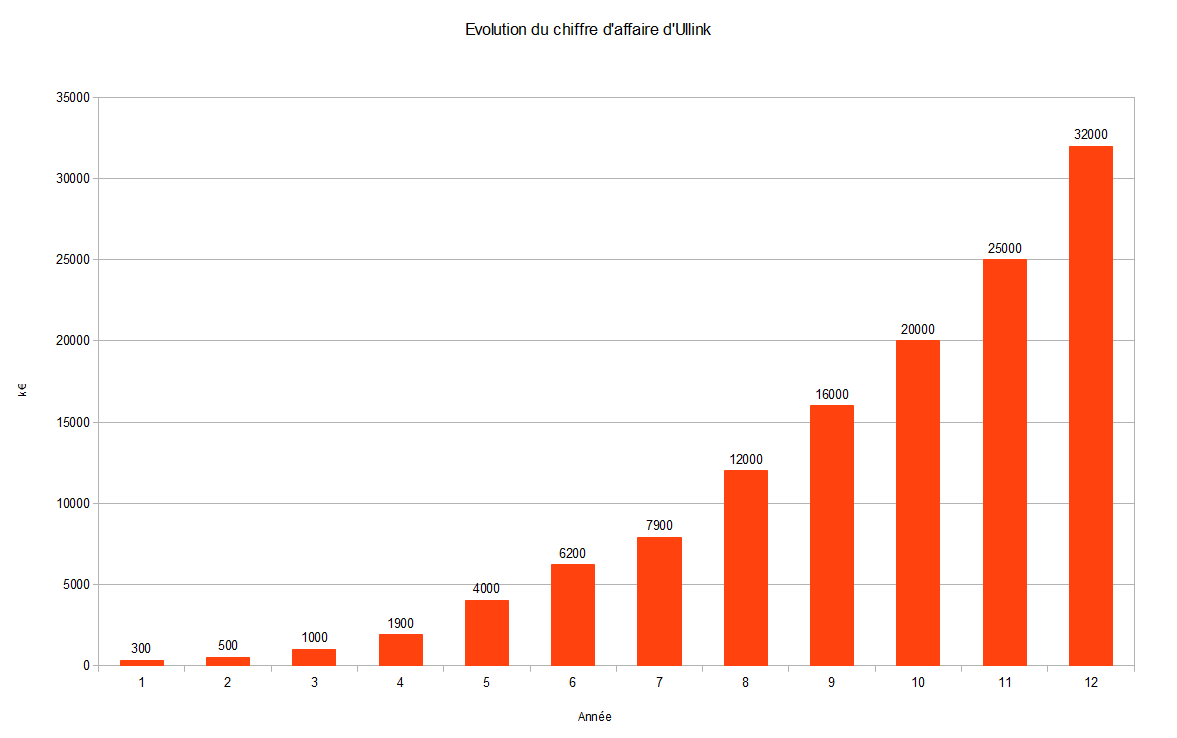
\includegraphics[width=\textwidth]{ca_ullink.png}
\caption{Evolution du chiffre d'affaire d'Ullink depuis sa création}
\label{ca_ullink}
\end{figure}

\subsection{Les marchés financiers}

Les marchés financiers sont des organisations permettant l'échange de produits financiers. Ces produits peuvent être des titres, comme des actions, ou des marchandises réelles, comme le pétrole ou le blé. Ils sont régulés par des autorités externes, comme l'\emph{AMF} en France, ou la \emph{SEC} aux Etats-Unis.

Quelques exemples de marchés sont \emph{NYSE}, \emph{EURONEXT} ou encore \emph{CME (Chicago Mercantile Exchange)}.\footnote{Plus d'informations sur les marchés financiers, ainsi que sur le vocabulaire associé peuvent être trouvés sur \url{http://www.investopedia.com/}}

\subsubsection{Les acteurs des marchés financiers}

\begin{figure}
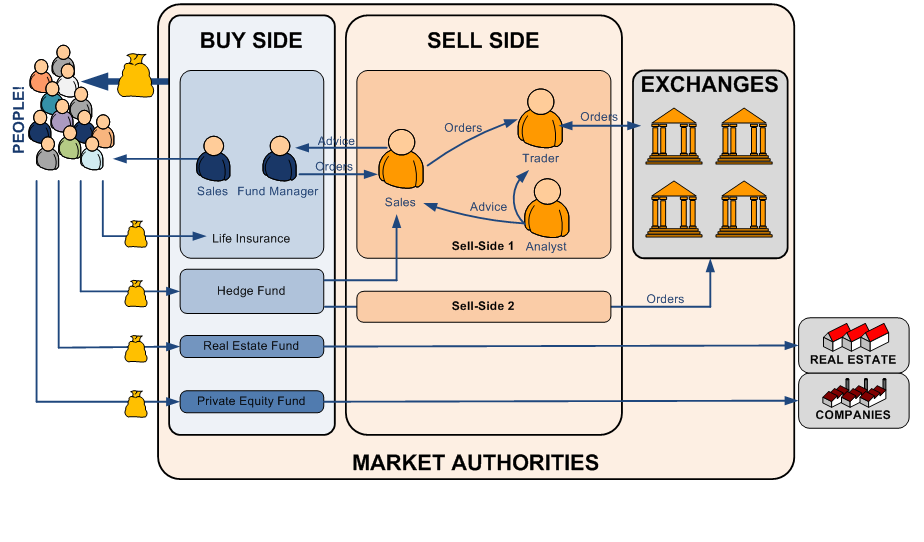
\includegraphics[width=\textwidth]{market_actors.png}
\caption{Les acteurs}
\label{market_actors}
\end{figure}

Il existe plusieurs acteurs dans les marchés financiers.

Principalement, il y a les \emph{buy-side} et les \emph{sell-side}. Les \emph{buy-side} sont contactés par les investisseurs, dans le but qu'ils fassent fructifier leur argent. Les \emph{sell-side}, sont les entités ayant un accès réel aux marchés, et conseillent les \emph{buy-side}. Les \emph{sell-side} se rémunèrent grâce aux commissions sur les ordres qu'ils exécutent pour les \emph{buy-side} sur les marchés.

Les buy side et sell sides ne sont pas les seuls acteurs du marché, mais ce sont ceux à qui sont destinés les produits Ullink.


\subsubsection{Les différentes actions possibles sur les marchés}

Bien qu'on ne puisse en théorie qu'acheter ou vendre sur un marché, il existe de nombreux types de valeurs, chaque type ayant ses spécificités, ce qui fait d'ailleurs toute la complexité du trading. Les \emph{equity} représentent des marchandises réelles, ou une action d'une société (\emph{ex: j'achète du pétrole, j'achète 10 parts AAPL}). Les \emph{derivatives}, représentent une action dérivée d'une marchandise (\emph{ex: j'achète le droit de vendre du pétrole dans 3 mois}). D'autres sont possibles, comme les \emph{debts}.

Une action de vente ou d'achat standard sur un marché est appellée \emph{trade}.

\subsection{Produits}

Ullink propose une suite logicielle de trading électronique ayant pour cible l'ensemble des acteurs sell-side et buy-side. L'accent est mis sur la robustesse et l'extensibilité.

Trois types de produits sont ainsi proposés, que nous allons voir dans les paragraphes suivants.

\subsubsection{Produits principaux}

\paragraph{UL Bridge}

UL Bridge permet la connexion client(s)/marché(s) de manière directe, ainsi que le routage des informations dans l'ensemble des produits des solutions Ullink.

\paragraph{UL Odysis}

UL Odisys sert à gérer des ordres plus complexes, ou nécéssitant intervention humaine. Ces ordres ne partirons pas directement sur les marchés, et seront traités par différents acteurs, avant de partir pour execution.

\paragraph{UL Desk}
UL Desk est la solution front-end principalement à destination des Traders et Brokers. Il facilite un bon nombre d'opérations, surtout les actions complexes, comme répartir un ordre entre plusieurs marchés. C'est une interface tout inclus permettant un niveau d'abstraction par rapport aux marchés. Ses fonctionalités sont fournies par des extensions, comme ul-trader, pour les traders.

\subsubsection{Solutions complémentaires}
Un certain nombre d'autres composants logiciels sont disponibles pour offrir un ensemble de fonctionalités plus riche:

\begin{itemize}
\item{\textbf{UL Smart} est une couche d'automatisation permettant la recherche des meilleures exécutions possible lors des passages d'ordres.}
\item{\textbf{UL Iris} implémente une gestion des risques avant le passage réel d'un ordre sur les marchés.}
\item{\textbf{UL Dashboard} permet d'avoir une vision d'ensemble de l'intégralité des activités réalisée sur la plateforme Ullink, du point de vue technique.}
\item{\textbf{UL Monitoring} offre une vision métier des opérations réalisées sur la plateforme Ullink.}
\end{itemize}

Il existe bien d'autres produits et plugins afin de permettre au client d'adapter leur solution à leurs workflows spécifiques.

Bien que Ullink propose dans ses produits des plugins permettant d'automatiser le trading dans une certaine mesure (UL Algo), Il n'y a pas de plan pour se lancer dans le HFT (High Frequency Trading)qui relève d'un mode de pensée à très court terme étant extrèmement préjudiciable à une entreprise\footnote{\url{http://www.huffingtonpost.com/2013/06/18/high-frequency-trading-profits_n_3459497.html} [EN]}.

\subsubsection{Hébergement}

En plus de son offre "classique" (hébergé et administrée par le client), Ullink propose aussi ses produits sous la forme d'un service managé, c'est à dire géré par Ullink, et mis à disposition du client via une connexion à distance. Ce type de solution présente l'avantage pour le client de ne pas avoir à se soucier des inconvénients liés à la gestion d'une solution logicielle, tels que les mises à jour, le choix des machines, et toutes les autres décisions techniques.

\subsection{Organisation}

Ullink est divisé en quatre départements majeurs (figure~\ref{depts_ullink}):

\paragraph{Produits}
Tout ce qui concerne les produits Ullink, de l'architecture à la démarche qualité, en passant par le développement.

\paragraph{Opérations}
Ce département est celui qui s'occupe des clients: réalistation de solutions, installation, support, gestion de portefeuille.

\paragraph{Business Development}
Secteur marketing, vision stratégique...

\paragraph{Services internes}
Comptabilité, RH, direction, IT interne.

\begin{figure}
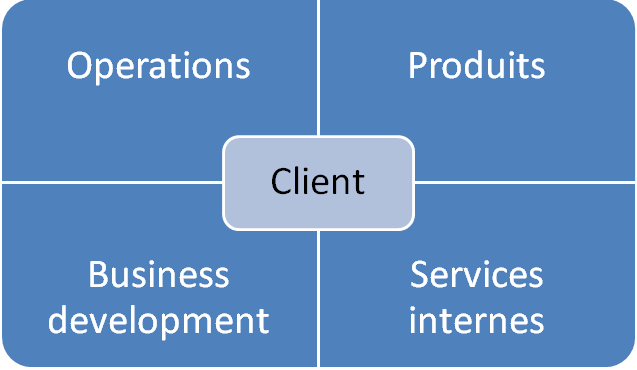
\includegraphics[width=\textwidth]{orga_deps_client.png}
\caption{Les départements chez Ullink}
\label{depts_ullink}
\end{figure}

\section{Activité au sein d'Ullink}

\subsection{Situation}

Je suis dans le département produit. Je forme avec mon camarade Sébastien ANTOINE, en IR3, l'équipe des Product tools\footnote{Renommée Build sur l'organigramme du département Produit en annexe (figure~\ref{Product_dpts_orga}).}. Nous sommes basés à Paris, dans un Open Space situé dans un immeuble du \textsc{\romannumeral 9}\textsuperscript{e}~arrondissement (voir Annexe).

Cette équipe se charge du développement et du maintien de l'environnement de travail propre au département Produit, en vue de faciliter l'utilisation dudit environnement par les équipes Produit.

Lors des jeunes années d'Ullink, un environnement de travail basé sur de l'intégration continue a été mis en place. Cet environnement faisait usage de plusieurs outils open source, dont le désormais célèbre serveur Hudson, repris par la suite sous le nom Jenkins. Ce serveur interagissait avec un serveur CVS, via un plugin personalisé par Ullink installé sur Jenkins. Ce plugin se chargeait aussi de gérer les scripts ant, permettant la construction des différentes solutions logicielles.

Cependant, ce qui était simple s'est complexifié avec le temps, le nombre de produits grandissant, les solutions spécifiques à tel client. L'équipe des Product Tools a donc été créée dans le but d'assurer la maintenance, et l'amélioration de ce système.

Dans ce cadre, nos sommes en contact avec toutes les différentes équipes du département Produit.

\subsection{Missions}
\subsubsection{Maintenance}

Notre mission de maintenance est claire: s'assurer que tous les éléments de la chaîne d'intégration continue -et les outils associés- fonctionnent correctement, de la manière la plus transparente possible pour les utilisateurs (les équipes de développement).

Ainsi, nous gérons la répartition des esclaves Jenkins parmis les différentes équipes et projets, installant ou retirant des esclaves si besoin. Nous nous occupons également des mises à jour des outils utilisés, et éventuellement de leurs optimisations.

\subsubsection{Développement}

Bien qu'une infrastructure soit déjà en place, des efforts pour migrer vers des outils plus puissants et/ou modernes doivent être faits. Nous avons rejoint le groupe de travail cherchant à migrer de \texttt{cvs} vers \git, ce qui rend une bonne partie des systèmes actuellement utilisés obsolètes. Ainsi, nous avons participé à la définition et mise en place d'un nouveau workflow, plus adapté au spécificités de \git, installé les différents outils logiciels permettant l'usage du workflow.

Par la suite, nous avons rédigé une documentation interne sur l'usage de \git. De plus, nous avons animé des formations \git à destination des équipes produit.

Une semi-automatisation des tâches de maintenance sur les nodes a également été développé, permettant une réduction du temps consacré à la maintenance afin de se concentrer davantage sur le développement.

Enfin, une automatisation plus poussée du processus de release a été développé par Sébastien, afin de tendre vers le continuous delivery.

\section{Valeurs d'entreprise}

\subsection{Management}

Ullink accorde une grande part à l'utilisation de la méthode de développement SCRUM\footnote{\url{http://fr.wikipedia.org/wiki/Scrum_\%28m\%C3\%A9thode\%29}}, les équipes sont invitées à être auto-organisées, et si possible auto-géréees.

Dans le cas de l'équipe des Product Tools, cela signifie que nous répondons également aux demandes des autres équipes, que ce soit par le système interne de gestion de tickets, ou une demande nous étant directement addressée. Nous sommes également ammenés à identifier les axes d'amélioration, de communiquer avec les autres équipes pour récolter leurs besoins, et de proposer un plan d'action. Il nous arrive aussi de travailler avec une (ou plusieurs) autre(s) équipe(s), et d'appliquer le scrum avec le(s) scrum master concerné(s).

\subsection{Collaboration}

Nous faisons un usage intensif d'outils de collaboration, tels que les wiki, afin de mettre en commun toutes les ressources dont nous disposons. Ceci est particulièrement utile pour les données administratives et de communication. Plusieurs espaces sont disponibles afin de regrouper les pages par thématique. il existe par exemple l'espae RH, l'espace architectes, l'espace produits...

La transparence et la communication font partie des valeurs clé d'Ullink.

\pagebreak
\section*{Conclusion}
\addcontentsline{toc}{section}{Conclusion}

Ullink est une entreprise encore jeune, pleine de dynamisme. Elle se donne les moyens de réussir. Sa plus grande réussite est selon moi d'avoir réussi à donner le sentiment qu'on peut faire bouger les choses, en tant qu'individu.

Cependant, de nombreux challenges restent à relever. De part son éclatement géographique, des efforts sont toujours nécessaires pour renforcer la collaboration entre les différents sites, et rendre l'expérience du développement chez Ullink plus agréable et simple. Efforts auquels je serai fier de participer dans les années à venir.

\pagebreak

\part*{Annexes}
\addcontentsline{toc}{section}{Annexes}
L'organigramme \ref{Product_dpts_orga} est disponible en grand à cette adresse: \url{https://raw.github.com/paulollivier/esipe-rapport-ir1/master/images/dep_product_orga.png}
\begin{figure}
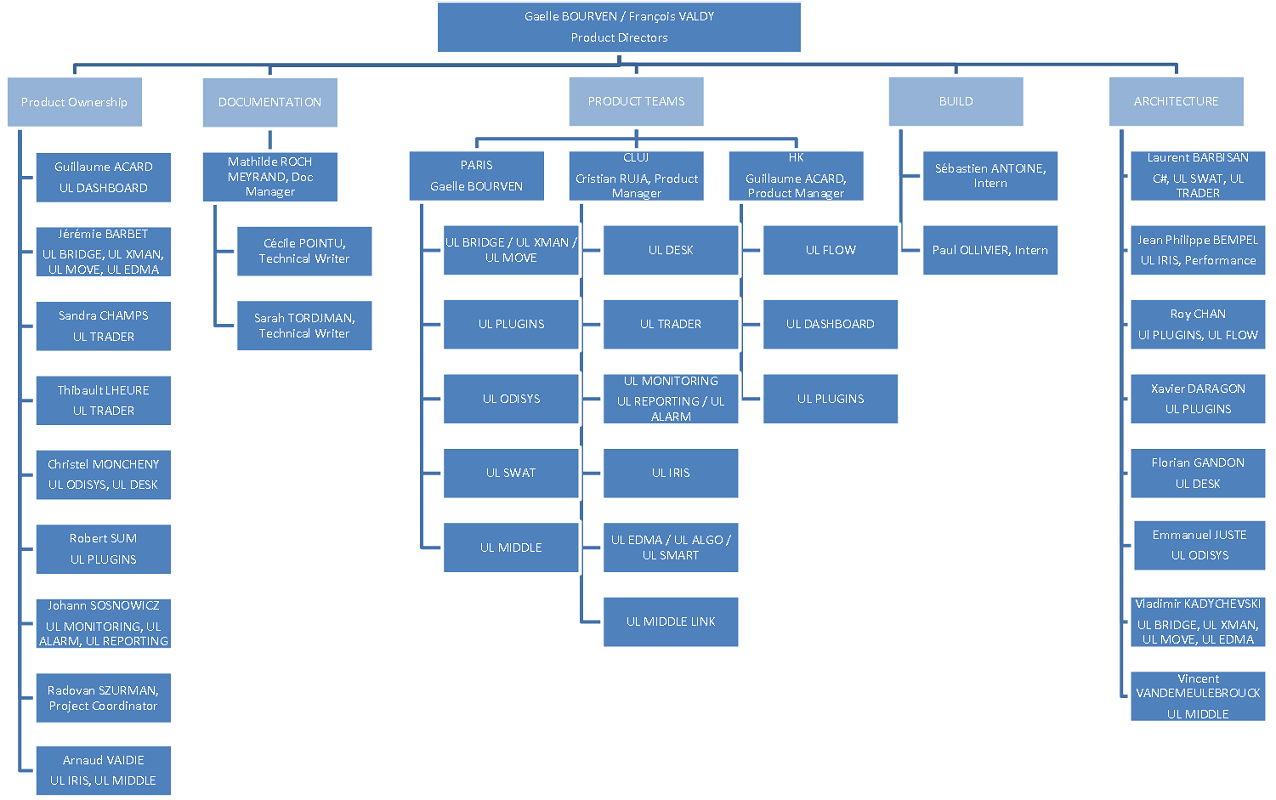
\includegraphics[width=525pt, angle=90]{dep_product_orga.png}
\caption{Organigramme département Produits}
\label{Product_dpts_orga}
\end{figure}

\begin{figure}
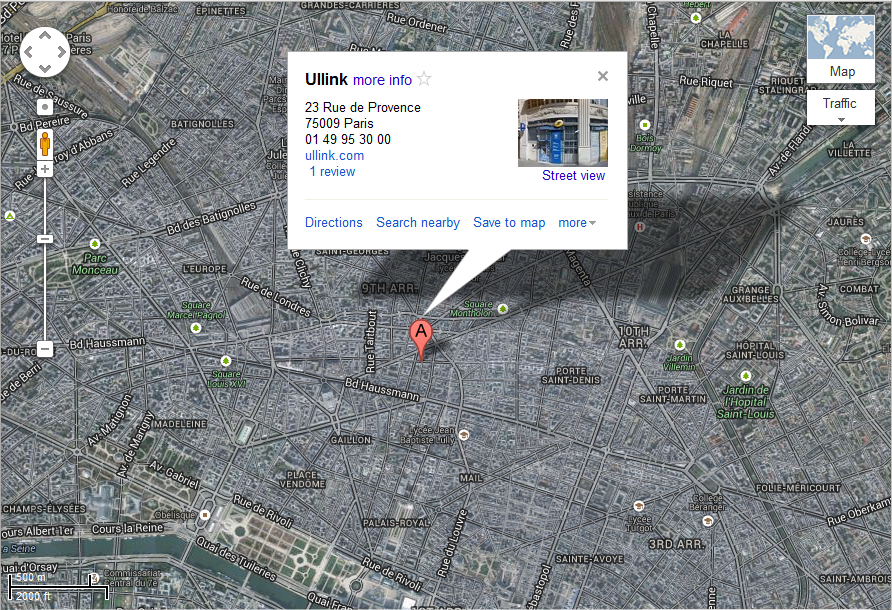
\includegraphics[width=\textwidth]{ullink_loc.png}
\caption{Situation géographique de Ullink Paris}
\label{ullink_loc}
\end{figure}

\begin{figure}
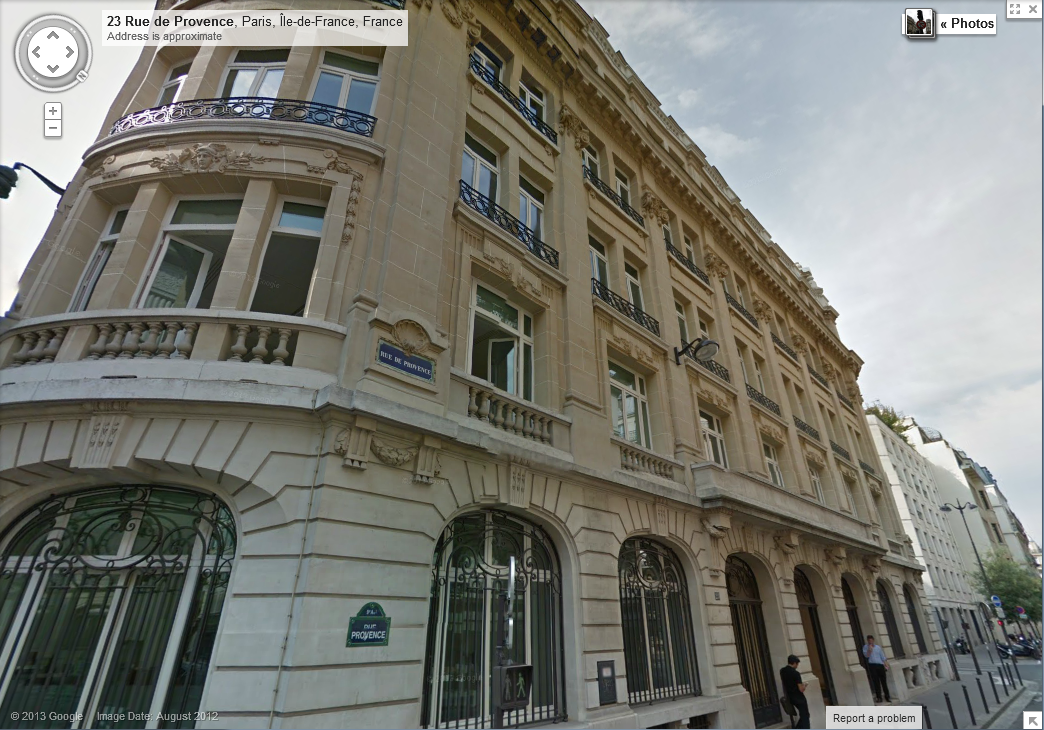
\includegraphics[width=\textwidth]{ullink_photo.png}
\caption{Photo de l'éxterieur des locaux de Ullink Paris}
\label{ullink_photo}
\end{figure}

\pagebreak

%!TEX root = rapport_ir1.tex
\begin{titlepage}
\begin{center}
\section*{Titre}
Ullink: une entreprise en pleine expansion

\section*{Résumé}
Présentation de l'entreprise Ullink, société éditrice de solutions de trading.

\section*{Mots clés}
\begin{multicols}{2}
\begin{itemize}
\item Développeur
\item Ullink
\item Environnement informatique
\item Logiciel
\item Trading
\item Méthodes Agiles/SCRUM
\end{itemize}
\end{multicols}



\vfill
les sources pour ce document sont disponibles sur \url{https://github.com/paulollivier/esipe-rapport-ir1}.
\end{center}
\end{titlepage}


\end{document}
